\documentclass[12pt]{article}
\twocolumn
\usepackage{graphicx}
%\documentclass[journal,12pt,twocolumn]{IEEEtran}
\usepackage[none]{hyphenat}
\usepackage{graphicx}
\usepackage{listings}
\usepackage[english]{babel}
\usepackage{graphicx}
\usepackage{caption}
\usepackage[parfill]{parskip}
\usepackage{hyperref}
\usepackage{booktabs}
%\usepackage{setspace}\doublespacing\pagestyle{plain}
\def\inputGnumericTable{}
\usepackage{color}                                            %%
    \usepackage{array}                                            %%
    \usepackage{longtable}                                        %%
    \usepackage{calc}                                             %%
    \usepackage{multirow}                                         %%
    \usepackage{hhline}                                           %%
    \usepackage{ifthen}
\usepackage{array}
\usepackage{amsmath}   % for having text in math mode
\usepackage{parallel,enumitem}
\usepackage{listings}
\lstset{
language=tex,
frame=single, 
breaklines=true
}
  
%Following 2 lines were added to remove the blank page at the beginning
\usepackage{atbegshi}% http://ctan.org/pkg/atbegshi
\AtBeginDocument{\AtBeginShipoutNext{\AtBeginShipoutDiscard}}
%
%New macro definitions
\newcommand{\mydet}[1]{\ensuremath{\begin{vmatrix}#1\end{vmatrix}}}
\providecommand{\brak}[1]{\ensuremath{\left(#1\right)}}
\providecommand{\abs}[1]{\left\vert#1\right\vert}
\providecommand{\norm}[1]{\left\lVert#1\right\rVert}
\newcommand{\solution}{\noindent \textbf{Solution: }}
\newcommand{\myvec}[1]{\ensuremath{\begin{pmatrix}#1\end{pmatrix}}}
\let\vec\mathbf
\begin{document}
\begin{center}
\title{\textbf{Parallel Lines}}
\date{\vspace{-5ex}} %Not to print date automatically
\maketitle
\end{center}
\setcounter{page}{1}
\section*{11$^{th}$ Maths - Chapter 10}
This is Problem-6 from Exercise 10.3
\begin{enumerate}
	\item Find the distance between parallel lines 
	
(i) 15x+8y-34=0 and  15x+8y+31=0 \\
(ii) l(x+y)+p=0 and  l(x+y)-r=0
\	
\item solution for problem 1

where
\begin{align}
&=\myvec{15&8}\vec{x}=-34\\ 
&=\myvec{15&8}\vec{x}=31\\
\vec{n}&=\myvec{15\\8},c_1=-34, c_2= 31
\end{align} 
distance between parallel lines 
\begin{align}
d&=\frac{\abs{c_1-c_2}}{\norm{\vec{n}}}\\
&=\frac{\abs{-34-31}}{\sqrt{289}}\\
&=\frac{65}{17}
\end{align}
\begin{figure}[h!]
\centering
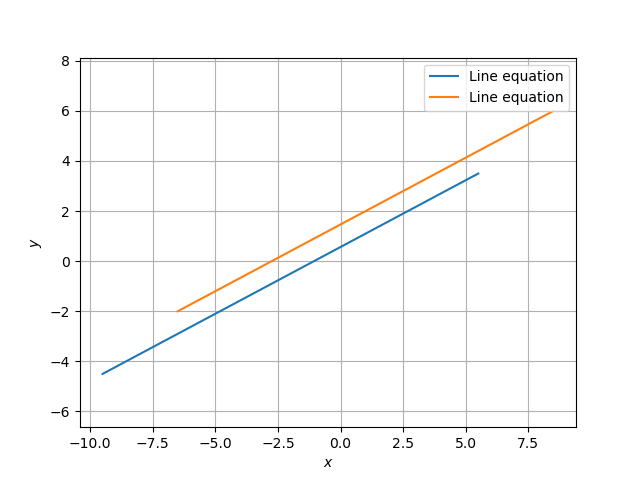
\includegraphics[width=\columnwidth]{../figs/para.png}
\caption{}
\label{fig:para.png}
\end{figure}
\
	\item solution for problem 2
	
 where
\begin{align}
\vec{n}&=\myvec{1\\1}\\
&=\myvec{1&1}\vec{x}=\frac{-p}{l}\\ 
&=\myvec{1&1}\vec{x}=\frac{-r}{l}		
\end{align}
distance between parallel lines 
\begin{align}
d&=\frac{1}{l\sqrt{2}}(p+r)
\end{align}	
The distance between parallel lines 
is shown in figure 2  with normal vector as 
\begin{align*}
&=\vec{n} =\myvec{1\\1} \text{ and }c_1=1,c_2=-1
\end{align*}
\begin{figure}[h!]
\centering
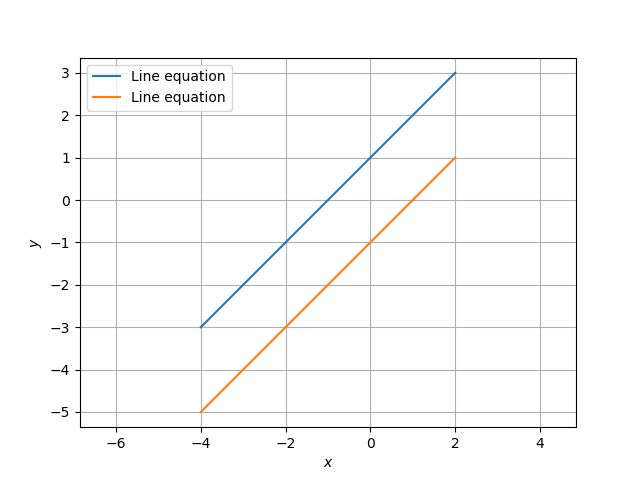
\includegraphics[width=\columnwidth]{../figs/para1.png}
\caption{}
\label{fig:para1.png}
\end{figure}
\end{enumerate}
\end{document}